\chapter{Diseño}
\label{sec:diseno}

%Es uno de los capítulos más importantes. Debe explicar claramente la solución propuesta justificando la aproximación adoptada. Este capítulo, según el caso, es aconsejable que defina claramente la arquitectura del sistema propuesto, identificando los roles o partes o actores del sistema. Pueden emplearse metodologías basadas en diagramas de clases, paquetes, diagramas secuenciales, diagramas de relación, etc.

%Si se ha diseñado una interfaz gráfica debe también describirse su estructura, dónde se mostrará la información, etc.


La figura \ref{fig:diag-bloques} muestra un diagrama con los bloques con el diseño general del proyecto. En el docker se incluye el \textit{deployer} que instala el \textit{core} de la cadena de bloques. Además, se encuentra la base de datos \texttt{postgresql}, que estará en interacción con el \textit{core} para almacenar y servir datos de las transacciones dentro de un nodo\cite{BD-ARK}.\\

Por otra parte, fuera del docker, se encuentra el \textit{explorer} y la aplicación Desktop Wallet. El \textit{explorer} estará conectado al \textit{core} mediante el puerto API $4200$, al \textit{explorer} se podrá acceder mediante un navegador con la dirección\mbox{\texttt{http://NODE\_GENESIS:4200}}. Sin embargo, para acceder a la aplicación Desktop Wallet será necesario descargarla, veáse apéndice manual de usuario \ref{sec:manual-wallet}, dicha apliación se conectará con el \textit{core} mediante el puerto API $4103$.

%Los nombres de la bases de datos se pueden ver con el comando psql -l, y podemos ver que hay una para cada red, a nosotros no interesa core_bridgechain_testnet. Para visualizar las tablas poner el comando psql -U deployer - d core_bridgechain_testnet.

\begin{figure}[H]
	\centering
	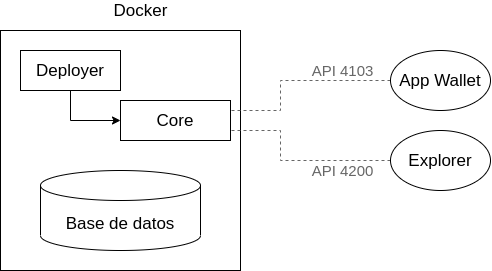
\includegraphics[width=0.8\textwidth]{figuras/diagrama_bloquesARK.png}
	\caption{Diagrama de bloques}
	\label{fig:diag-bloques}
\end{figure}


Finalmente, la estructura del algoritmo viene dada por un fichero escrito en python donde se encuentran las funciones que se explicarán en detalle en el capítulo \ref{sec:implementacion}. El fichero \texttt{uov.py} incorpora main con un ejemplo de uso del algoritmo independientemente de la \textit{blockchain}. Dicho fichero se encuentra alojado en el \textit{core} de la cadena de bloques para utilizarlo en el algoritmo de firma y verificación